\section{Persistent Data Storage}

As described previously, Capital Games is data-centric
and therefore cannot exist without a robust mechanism
for persisting user data between ``uses'' of the system.

Various methods exist for the persisting of data. They range
from serialization of system state variables into files
to storing all data in the form of elaborate relational
database systems, and anything in between. Capital Games
primarily makes use of relational and non-relational databases.

In a relational database, stand-alone sets of data are placed
into indexed tables stored in computer memory, with each row in a table
representing a single set and each column representing a single
attribute. A table can have a very large (sometimes even 
infinite) number of columns and rows. A database possesses
many interrelated tables which are cross referenced by their
indices (called primary and foreign keys). These relations
allow complex queries against tabulated data. \cite{wiki:rdb}

\begin{figure}[ht]
\centering
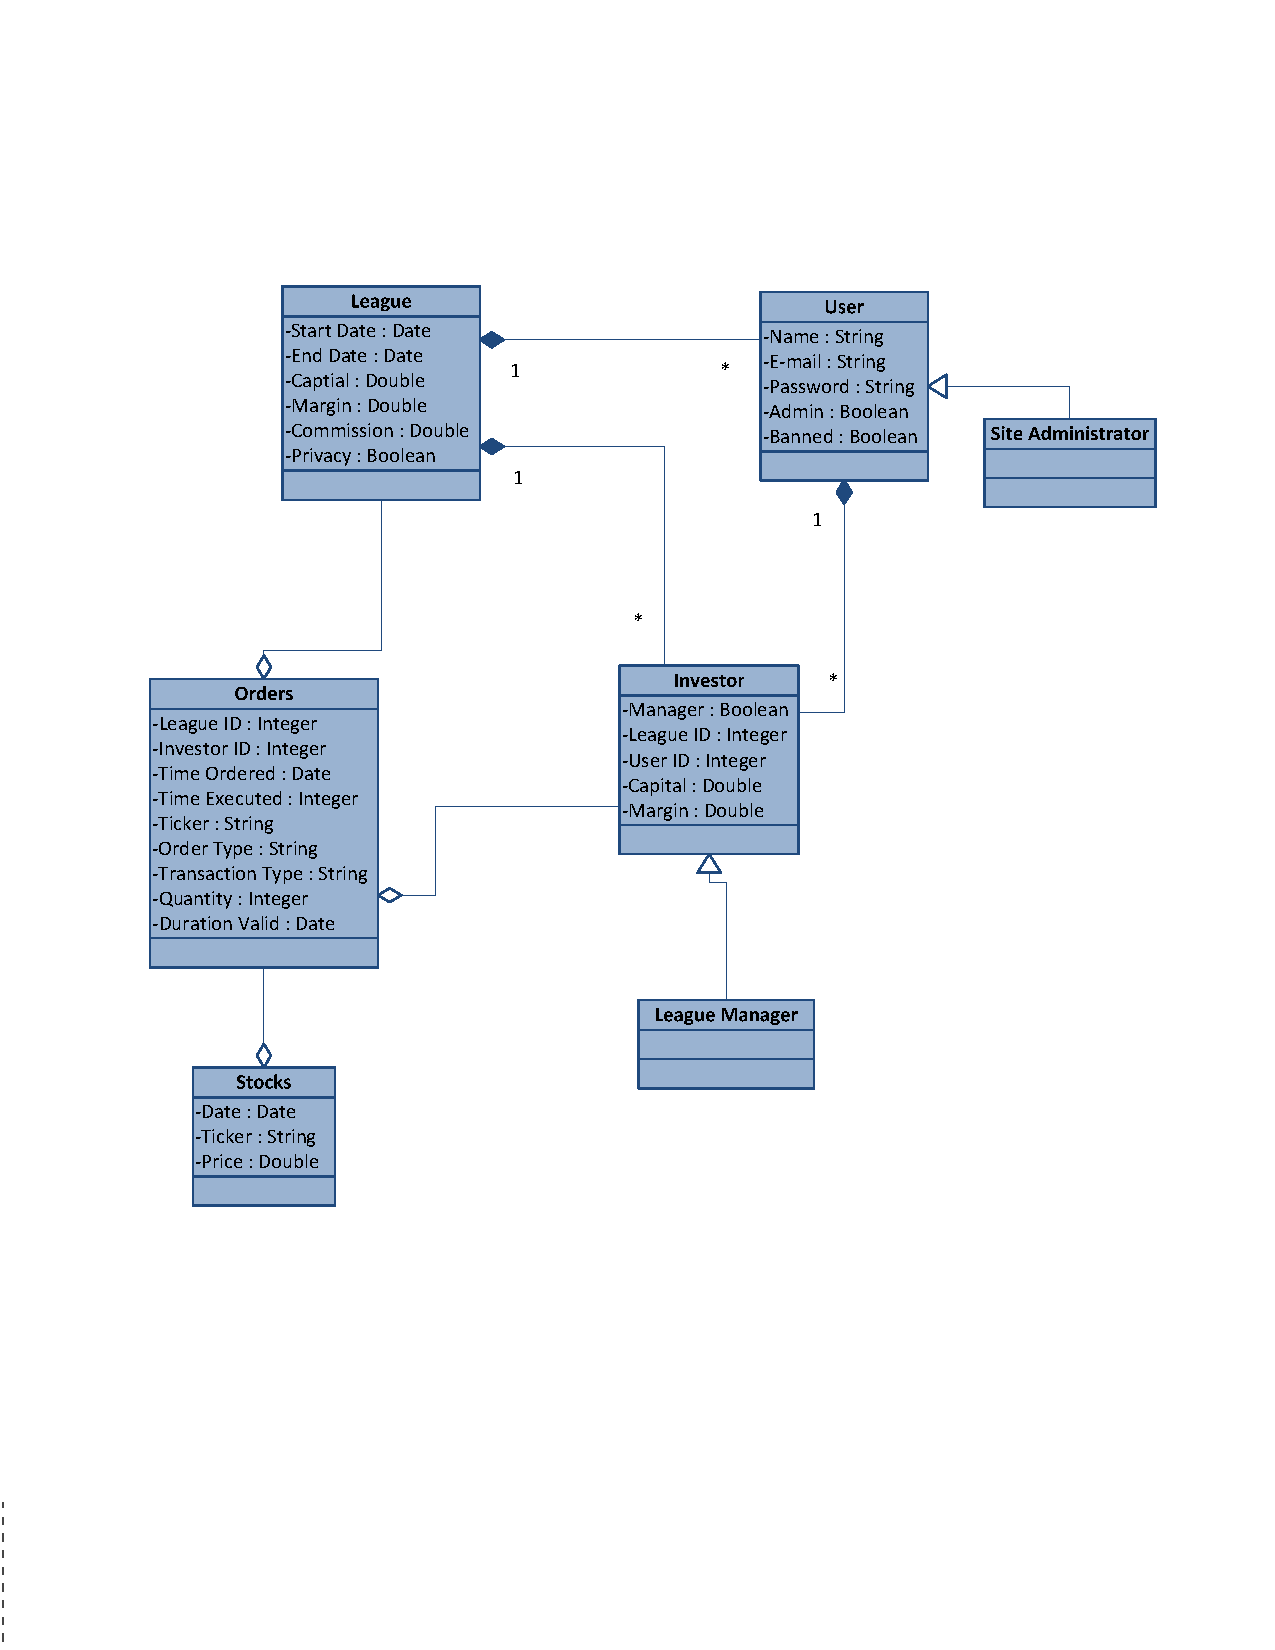
\includegraphics[width=6in]{./img/domainModel.pdf}
\caption{The format of the relational database
schema implemented by Capital Games for its core features.
(Not comprehensive.)}
\end{figure}

For example, consider the figure shown previously, repeated here.
A league is the most fundamental data structure of Capital games,
yet it is not aware of its users, their portfolios, or of any
orders associated with them. To retrieve these data, a query can
be performed which pivots around the indices relating the tables.
To find out a list of users participating in a league, one could
take that league's index (not shown in figure for brevity) and
search for all investors with that index; then take the user
indices contained in the resulting query and dereference them
to identify the original users. 

Additionally, Capital Games makes use of a so-called ``NoSQL'',
or non-relational database. The format of such a database is
practically unrestricted, and data need not belong in tabular
format. This approach exchanges speed and scalability for
querying power. \cite{wiki:nosql} Capital Games utilizes the
Redis NoSQL database to store outstanding queued jobs. This
structure was chosen so that the database store can be
seamlessly scaled across many machines if need be, and
because of its light weight. 